% ./build.sh to compile
\documentclass[convert={density=300,size=400x400,outext=.png}]{standalone}
\usepackage{tikz}
\usetikzlibrary{shapes.geometric,positioning}
\usetikzlibrary{calc}
\begin{document}
  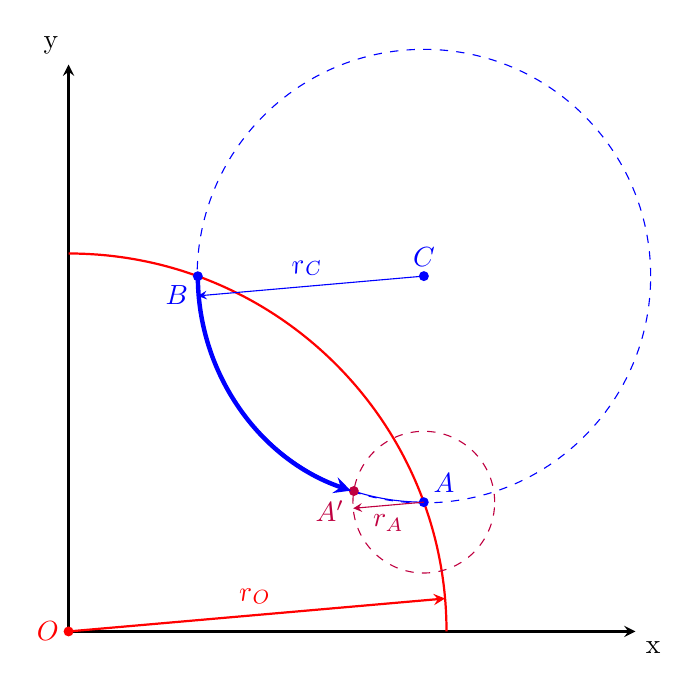
\begin{tikzpicture}[>=stealth,scale=1.2]
    % Axes
    \draw[thick,->] (0,0) -- (6,0) node[anchor=north west] {x};
    \draw[thick,->] (0,0) -- (0,6) node[anchor=south east] {y};
    % O
    \draw[red,thick] (4,0) arc (0:90:4);
    \coordinate[label=left:$\textcolor{red}{O}$] (O) at (0,0);
    \fill[red] (O) circle [radius=1.5pt]; 
    \draw[red,thick,->] (0,0) -- node[above, rotate=5] {$\textcolor{red}{r_O}$} (5:4);
    % A
    \coordinate [label=above right:$\textcolor{blue}{A}$] (A) at (20:4);
    \fill[blue] (A) circle [radius=1.5pt]; 
    % B
    \coordinate [label=below left:$\textcolor{blue}{B}$] (B) at (70:4);
    \fill[blue] (B) circle [radius=1.5pt]; 
    % A-B circle
    \draw[blue] (A) arc (270:180:2.4);
    % C center
    \coordinate[label=above:$\textcolor{blue}{C}$] (C) at (3.76,3.76);
    \fill[blue] (C) circle [radius=1.5pt]; 
    \draw[dashed,blue,thin] (C) circle [radius=2.4];
    % C arrow
    \draw[blue,->] (C) -- node[above, rotate=10] {$\textcolor{blue}{r_C}$} ++(185:2.4);
    % A' center
    \coordinate [label=below left:$\textcolor{purple}{A'}$] (A') at ($ (A) + (171:0.75) $);
    \fill[purple] (A') circle [radius=1.5pt]; 
    % A' circle
    \draw[dashed,purple,thin] (A) circle [radius=0.75];
    % A' arrow
    \draw[purple,->] (A) -- node[below] {$\textcolor{purple}{r_A}$} ++(185:0.75);
    % Final result
    \draw[blue,ultra thick,->] (B) arc (180:251:2.4);

  \end{tikzpicture}
\end{document}
